\subsubsection{AVL}
\begin{figure}[H]
    \centering
    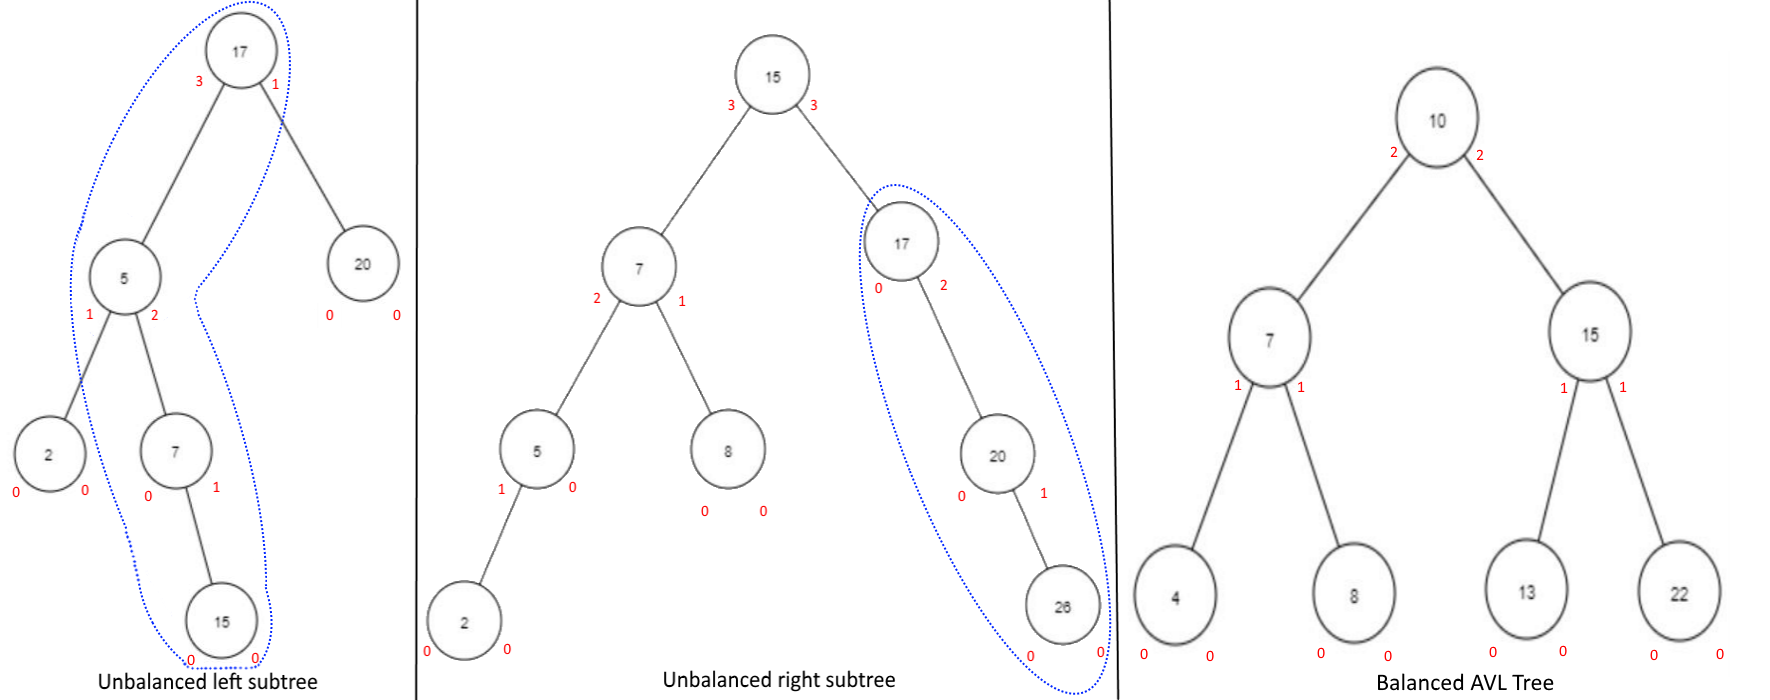
\includegraphics[width=0.90\linewidth]{/trees/AVLTreesVer2}    
    \caption{The figure displays 2 unbalanced binary search trees and a fully balanced AVL tree. }
    \label{fig:AVLTrees}
\end{figure}
\noindent
An example of balanced and unbalanced BSTs can be seen in figure \ref{fig:AVLTrees}. The left tree is a BST that has too many nodes in the left subtree. The center tree is a BST that has too many nodes in the right subtree. The tree to the right in the figure is a fully balanced BST, which makes it qualified as an AVL tree. The red letters represent the height of the node's children. The value is determined by how many nodes there are between the leaf nodes to the selected node. The blue dotted lines mark the subtree that breaks the AVL condition.
\\[11pt]
In this project, the name of the rotation direction is based on which subtree side has the most nodes. This means that in the previous example\ref{fig:AVLTrees}, the middle tree, a right rotation was needed that would have rotated the right subtree one step to the left. The opposite happens in a left rotation; too many nodes in the left subtree will make it rotate in the right direction. In some circumstances, a double rotation is needed. These, on the other hand, are named after the last direction the nodes need to rotate in order to balance the subtree. Double left rotation means that a rotation towards the right is first used on the right child of the node causing the imbalance. This switches the right child's spot with the imbalanced node. Then followed by a rotation on the new imbalanced node towards the left. The opposite will occur on a double right rotation.
\\[11pt]
The function \code{createAVLTreeSolution} creates an AVL tree used as the solution object for a question. The functionality is mostly the same as the \code{createBinarySearchSolution} function mentioned earlier. However, some extra functionality was needed in order to balance the tree. If an existing tree is given, the given tree needs to be fully balanced before any insertions or deletions can be done to the tree. Once the existing tree is balanced or no existing tree was given, the values in the added array are inserted in the tree. Just like in \code{createBinarySearchSolution}, removing nodes from a tree requires that an existing tree is given. After every insertion and deletion, the tree will once again have to be checked to see whether or not it is still balanced. If the tree is not balanced, the tree will have to rotate in order to rebalance itself. The rotation is determined by which subtree currently has the most nodes. Not to mention insertion and deletion require a different set up when it comes to using normal rotation or double rotations. The returning array from the \code{createAVLTreeSolution} is used and has the same format as in the \code{createBinarySearchSolution} function. The only noticeable difference is that the array for the \code{createAVLTreeSolution} also need to store the tree state after any rotations have been performed.
\\[11pt]
Because the \code{Tree} class contained circular references between a parent node and child nodes, it proved difficult to store solution BSTs and AVL trees into the database. This was because it was not possible to convert the tree object to JSON, since JSON cannot handle circular references. This means that the circular references had to be removed before the solution could be stored in the database. To solve this an export function was implemented for the \code{Tree} class. The export function removes the circular references by turning the parent reference into the parent's node value. Once the parent reference is gone, the tree object was able to be converted to JSON format. Of course, since the solution checker requires BSTs and AVL trees to be in a certain format, an import function also needed to be used to convert the tree object back to its original form. The import function has two tasks. The first task is to replace all null values with an undefined value. The second job is to reinsert the proper parent reference to each node in the tree. This is simply done by traversing the tree and remembering the previously visited node as the current node's parent. Once this is done the solution object can be checked with the converted tree the students drew with the GraphDrawer and see if they match or not. If the question revolved around removing nodes, then the converted tree only needs to match one of the trees in the solution object.

